\chapter[Optical spatial MIMO: System using imaging receiver]{Optical MIMO system using imaging receiver}
\label{chapter:mimoSpace}
\thispagestyle{myheadings}
%This chapter explores the spatial dimension to create an optical MIMO channel. It investigates the imaging receiver to effectively decorrelate spatially separated sub--channels. A normalization framework for OWC systems with imaging receiver is then outlined. Significant performance enhancements for spatial modulation and spatial multiplexing are shown by using an imaging receiver \cite{but14a}. SIS-OFDM, a novel modulation technique the utilizes the spatial dimension afforded by using multiple luminaires is then outlined \cite{but14b}. It incorporates simplicity of SM along with spectral efficiency of O-OFDM into one optical MIMO modulation technique.

Spatial modulation (SM) and spatial multiplexing (SMP) are two MIMO techniques for transmitting data over an indoor optical wireless channel. Receivers for SM and SMP can be of the non--imaging type, in which case the channel matrix coefficients can be highly correlated, or of the imaging type, which can reduce the degree of correlation and improve overall system performance. In this chapter, we propose a novel framework to analyze the performance of imaging MIMO systems. This framework is applied to characterize the performance of SM and SMP under both imaging and non--imaging receivers. Results of our analysis indicate that imaging receivers can provide significant SNR improvements of up to 45 dB under SM and SMP as compared to the use of non--imaging receivers. Finally, the application of the proposed analysis framework indicates specific design principles to optimize imaging receiver parameters\footnote{This work is published in peer--reviewed IEEE conference proceeding \cite{but14a}.}. 

% -------------------------------------
% SECTION: Channel with imaging receiver
% -------------------------------------
\section{Optical MIMO system with imaging receiver}
\label{sec:mimoImaging}

\graphicspath{{_MIMOSpace/figures_mimoImg/}}
In this section, an optical MIMO imaging system as illustrated in \figurename{ \ref{figMIMOblock}} is considered. Multiple luminaires are located near the ceiling of an indoor space to provide illumination and act as transmitters for communication. Information to transmit is jointly coded across a set of luminiares within the FOV of the receiver. User requested illumination state sets the average radiant flux emitted by the transmitters. Based on these inputs, the modulator generates drive signals for each luminaire. LEDs in the luminaire convert modulated data in the electrical domain into optical signals in the visible spectrum (E/O and conversely O/E conversion). These optical signals propagate through the indoor space and are incident on the receiver. 

\figurename{ \ref{figImagingReceiver}} illustrates a schematic of an imaging receiver. An imaging receiver for OWC can be modeled as a sensor and imaging optics. The sensor is located at a distance $f$ away from the optical center of the lens and is comprised of a grid of detector elements - each referred to as a `pixel'. Each pixel is comprised of a filter and optical detector. The imaging optics redirect light rays originating from different of an irradiating planar surface such that they are incident on corresponding different locations on the sensor. In other words, based on the angle and the location of incidence, light rays are redirected by the imaging optics on to a specific path. Thus it can extract and isolate optical signals originating from different spatial locations that get mixed while propagating through the indoor space. This helps to decorrelate signals received from spatially distinct transmitters and help significantly improve communication performance. Similarly, the ambient radiant flux incident at the aperture of the receiver is distributed among all pixels of the sensor. This helps to significantly reduce shot noise per pixel \cite{dja00a}. The receiver uses all received streams to jointly decode and recover information. 
\begin{figure}[t]
	\centering
		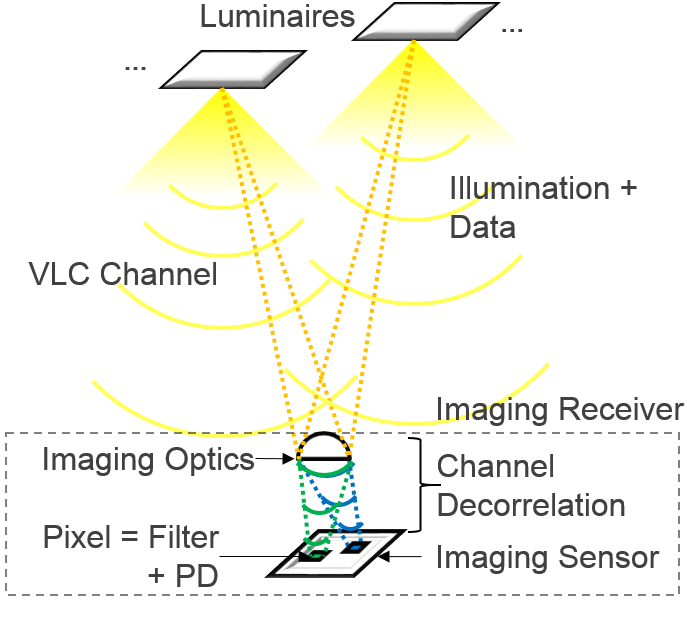
\includegraphics[trim={0.5in 0.25in 0.5in 0.25in}, clip=false, width=2.8in]{figMIMOmodel2.png}
	\caption{Optical MIMO system with imaging receiver}
	\label{figMIMOblock}
\end{figure}
\begin{figure}[b]
	\centering
		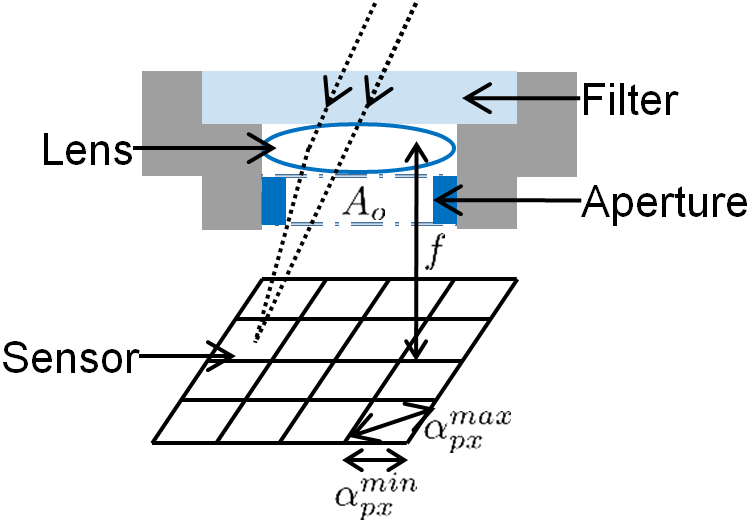
\includegraphics[width=3in]{figImagingReceiver.png}
	\caption{Schematic of an imaging receiver}
	\label{figImagingReceiver}
\end{figure}

Let $N_{\text{tx}}$ represent number of luminaires using which information is transmitted to user and let $N_{\text{px}}$ represent number of contiguous pixels comprising the sensor of an imaging receiver. The optical $N_{\text{tx}} \times N_{\text{px}}$ MIMO system can be represented by
\begin{equation}
	\label{eqMimoChannel3}
	\bf{Y} = \bf{H}\bf{X} + \bf{W}
\end{equation}
$\bf{X}$ is a $N_{\text{tx}}$ dimensional vector whose each element is the signal radiant flux emitted by each transmitter. The flux propagates over multiple paths before being incident on the imaging optics. As discussed in the SISO system, the LOS component of received flux is dominant over the NLOS component due to additional propagation and non--ideal reflection losses . $\bf{H}$ is a $N_{\text{px}}\times N_{\text{tx}}$ dimensional channel gain matrix where each element or channel gain coefficient $h_{ij}$ indicates the net channel gain from transmitter $j$ to pixel $i$. $\bf{W}$ is a $N_{\text{px}}$ dimensional noise vector. For imaging receivers, the shot noise at each pixel due to ambient illumination is severely diminished \cite{dja00a} and thus TIA input noise current is dominant source of noise \cite{kah97a}. For imaging receivers, ${\bf{W}}\sim\mathcal{N}({\bf{0}}$, $\sigma_{n}^2{\bf{I}})$ where $\sigma_{n}^{2}$ equals total noise current density. $\bf{Y}$ is a $N_{\text{px}}$ dimensional vector whose each element is the output signal current from each pixel.

For each individual link between transmitter $j$ and pixel $i$, the free space gain is defined as the fraction of the radiant flux emitted by the transmitter that is incident on the receiver aperture. Let [$x_{j}$ $y_{j}$ $z_{j}$] be the location of centroid $C_{j}$ of the illumination surface of the $j^{th}$ transmitter and [$x_{\text{rx}}$ $y_{\text{rx}}$ $z_{\text{rx}}$] be the location of the centroid of the receiver aperture. Optical axis ($\vm{d}_{j}$) between transmitter $j$ and receiver can be computed from Eq. \eqref{eqOpAxis}. The free space channel gain is then given by
\begin{equation}
	\label{eqMimoHFS}
	h^{\text{fs}}_{j} = L_{j}(\phi_{j})\frac{A_{\text{o}}}{||{\bf{d}}_{j}||^2}cos(\psi_{j})
\end{equation}
$\phi_{j}$ is the angle subtended between the optical axis and surface normal of the transmitter. $L_{j}(.)$ is the Lambertian radiant intensity as given by Eq. \eqref{eqLambertian}. Let $A_{\text{o}}$ be the area of the aperture opening. $\psi_{j}$ is the angle between the optical axis and surface normal of the receiver.

The magnification property of imaging optics determines the point of incidence on the sensor for a ray of light originating from the irradiating surface of the transmitter. Using ray tracing methods for a point aperture, it can be mathematically represented by
\begin{equation}
	\label{eqOpMag}
	M_{\text{im}} = \twopartdef {\frac{f}{||{\bf{d}}_{j}^{z}||-f}} { \psi_{j}\leq\psi_{c}^{rx}} {0} { \psi_{j}>\psi_{c}^{rx}}
\end{equation}
$f$ is the focal length of the imaging optics. $\psi_{c}^{rx}$ is the FOV of the receiver. Depending on the sensor dimensions, this may be smaller than or equal to the FOV of imaging optics.
Assuming the receiver is focused on the transmitter, the location of $C_{j}$ as projected in the RCS is given by
\begin{equation}
	\label{eqLocSp}
	{\vectthree{x_{\text{sp}}}{y_{\text{sp}}}{z_{\text{sp}}}}_{j} = \vectthree{-M_{\text{im}}({\bf{d}_{j}}.{\hat{\bf{x}}})}{-M_{\text{im}}({\bf{d}_{j}}.{\hat{\bf{y}})}}{-f}
	\end{equation}
	
Assuming the mathematical model of the shape of the luminaire's illumination surface is known, the shape of its projected spot on the plane of surface of the sensor can be calculated. Depending on the geometry of the transmitters and receiver, a pixel may receive light from multiple spots. Accordingly, the system performance gets severely degraded due to  the correlated channel matrix coefficients and inter channel interference (ICI). Non-polygonal shapes can be approximated to a polygon with very small error. Polygon itersection algorithms can be used to compute the shared area between a spot and pixel. The imaging channel gain (\ref{eqMimoHIm}) between transmitter $j$ and pixel $i$ is then given by the ratio of the fraction of the area of the spot $j$ that is incident on pixel $i$ to total area of the spot $j$.
\begin{equation}
	\label{eqMimoHIm}
	h^{\text{im}}_{ij} = \frac{\text{Area}(\text{spot}_{j}\cap \text{pixel}_{i})}{\text{Area}(\text{spot}_{j})}
\end{equation}
%\begin{equation}
	%\label{eqMimoHIm}
	%h^{\text{im}}_{ij} = \twopartdef{1}{\text{ spot$_{j}$ inside pixel i}}{0}{\text{ otherwise}}
%\end{equation}

Let $S_{j}(\lambda)$ be the SPD of the flux over link $j$ and $T_{i}(\lambda)$ and $R_{i}(\lambda)$ be the filter transmittance and responsivity at pixel $i$ respectively. The optical filter transmittance in this case is assumed independent of the angle of incidence of the flux. Let $Q$ be the transmittance of the imaging optics. The effective responsivity of pixel $i$ over link $j$ is given by
\begin{equation} 
	\label{eqPxResp}
	R_{ij} = Q\int_{\lambda_{min}}^{\lambda_{max}}S_{j}(\lambda)T_{i}(\lambda)R_{i}(\lambda)d\lambda
\end{equation}

Thus the net channel gain matrix $\bf{H}$ can be computed from the free space channel gain, the imaging channel gain and effective pixel responsivity by
\begin{equation}
	\label{eqMimoH}
	{\bf{H}}(i,j) = h_{ij} = h^{\text{fs}}_{j}h^{\text{im}}_{ij}R_{ij}
\end{equation}
where element $h_{ij}$ is the net channel gain from transmitter $j$ to pixel $i$.



% -------------------------------------
% SECTION: Imaging receiver framework
% -------------------------------------
%%%%%%%%%%%%%%%%%%%%%%%%%%%%%%%%%%%%%%%%%%%%%%%%%%%%%%%%%%%%%%%%
%%%%%%%%%%%%%%%%%%%%%%%%%%%% OSM IMG %%%%%%%%%%%%%%%%%%%%%%%%%%%
%%%%%%%%%%%%%%%%%%%%%%%%%%%%%%%%%%%%%%%%%%%%%%%%%%%%%%%%%%%%%%%%
\section{Imaging receiver normalization framework}
\label{sec:mimoImagingFramework}
\graphicspath{{_MIMOSpace/figures_osm/}}

It is desired to analyze the effect of imaging receiver configuration on performance of optical MIMO modulation techniques. The system performance is dependent on how the transmitter images or `spots' land on the sensor. Different system configurations can generate similar spot profiles on the sensor and thus similar communication  performance. To analyze the OWC system performance independent of a specific system configuration, the following normalization parameters are defined.

\subsubsection{Normalized luminaire side length}
\label{subsubsec:frameworkSide}
The normalized luminaire side length $\alpha_{\text{s}}$ is defined as the ratio of the length of the longest segment across a spot to side length of a pixel. 
\begin{equation}
	\label{eqAlphaS}
	\alpha_{\text{s}} \triangleq \frac{M_{\text{im}} a_{\text{tx}}^{\text{max}}}{\alpha_{\text{px}}^{\text{min}}}
\end{equation}
where $a_{\text{tx}}^{\text{max}}$ is the length of longest segment across irradiating surface of the luminaire. $\alpha_{\text{s}}$ specifies the spot size relative to the sensor dimensions. For example, consider two similar systems which differ in only the luminaire diagonal and PD side lengths. If both parameters differ in scale by the same factor, $\alpha_{\text{s}}$ would remain the same for both systems. $\alpha_{\text{s}}\leq 1$ implies the spot size is at most as large as the size of a PD. If the centroid of the spot is aligned with the centroid of a PD, the spot will lie completely inside the PD.
 
\subsubsection{Normalized luminaire pitch}
\label{subsubsec:frameworkPitch}
The normalized luminaire pitch $\delta_{\text{s}}$ is defined as the ratio of the spot-spot pitch to the length of the longest segment across the pixel. 
\begin{equation}
	\label{eqDeltaS}
	\delta_{\text{s}} \triangleq \frac{M_{\text{im}} P_{\text{tx}}}{\alpha_{\text{px}}^{\text{max}}}
\end{equation}
where $P_{\text{tx}}$ is the luminaire-luminaire pitch. $\delta_{\text{s}}$ specifies the distance between the centroids of adjacent spots relative to the sensor dimensions. For example, consider two similar systems which differ in only the transmitter pitch and PD diagonal. If both parameters differ in scale by the same factor, $\delta_{\text{s}}$ would remain the same. $\delta_{\text{s}}>1$ ensures that centroids of adjacent spots lie on different pixels. In the limit, if both transmitters were point sources, condition $\delta_{\text{s}}>1$ would ensure that different pixels receive signals from neighboring transmitters, thus eliminating ICI.

\subsubsection{Normalized luminaire edge-edge distance}
\label{subsubsec:frameworkEdge}
The normalized luminaire edge-edge distance $\eta_{\text{s}}$ is defined as the ratio of minimum distance between the edges of adjacent spots to the length of the pixel diagonal.
\begin{equation}
	\label{eqEtaS}
	\eta_{\text{s}} \triangleq \frac{M_{\text{im}}(P_{\text{tx}}-\alpha_{\text{tx}}^{\text{max}})}{\alpha_{\text{px}}^{\text{max}}}
\end{equation}
$\eta_{\text{s}}$ specifies the minimum possible distance between the edges of adjacent spots relative to the sensor dimensions. For example, now consider two similar systems which differ in only the minimum possible distance between the edges of adjacent luminaires and PD diagonal. If both parameters scaled by the same factor, $\eta_{\text{s}}$ would remain the same. $\eta_{\text{s}}>1$ ensures that adjacent spots do not overlap on any pixel. $\eta_{\text{s}}$ can be expressed in terms of $\alpha_{\text{s}}$ and $\delta_{\text{s}}$ as in (\ref{eqES2}). For square pixels, $l=1/\sqrt{2}$.

\begin{align}
	l &= \frac{\alpha_{\text{px}}^{\text{min}}}{\alpha_{\text{px}}^{\text{max}}}\label{eqESl}\\
	\eta_{\text{s}} &= \delta_{\text{s}} - l\alpha_{\text{s}}\label{eqES2}
\end{align}

\subsubsection{Normalized magnification}
\label{subsubsec:frameworkMagnification}
Let $M_0$ be the magnification of the system when $\alpha_{\text{s}}=1$. Normalized magnification is defined as the ratio of the magnification of the system to $M_0$.

\begin{align}
	M_{0} &\triangleq \frac{\alpha_{\text{rx}}^{\text{min}}}{\alpha_{\text{tx}}^{\text{max}}}\label{eqM0}\\
	\mu_{\text{s}} &\triangleq \frac{M_{\text{im}}}{M_{0}}\label{eqMS}
\end{align}
Consider two similar systems that differ in distance between the luminaire plane and the receiver and also in the receiver focal lengths. $\mu_{\text{s}}$ for both systems is the same value when both parameters differ in scale by the same factor.

% -------------------------------------
% SECTION: Spatial Modulation
% -------------------------------------
\section{Optical spatial modulation and multiplexing}
\label{sec:osm}

\graphicspath{{_MIMOSpace/figures_osm/}}

\subsection{Spatial modulation and spatial multiplexing}
\label{subsec:osmSystem}

\begin{figure}[t]
	\centering
		\begin{subfigure}{0.49\textwidth}
		\centering
				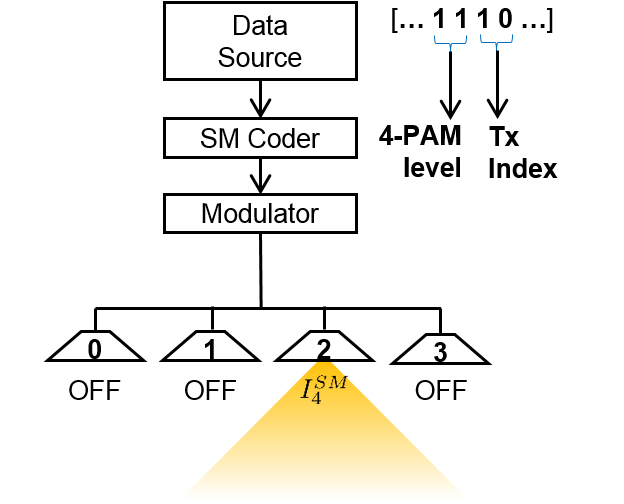
\includegraphics[trim=0in 0in 0in 0in, clip=false, width=2.5in]{figSM.png}
		\caption{}
		\label{figSM}			
		\end{subfigure}
		\hfill
		\begin{subfigure}{0.49\textwidth}
		\centering
				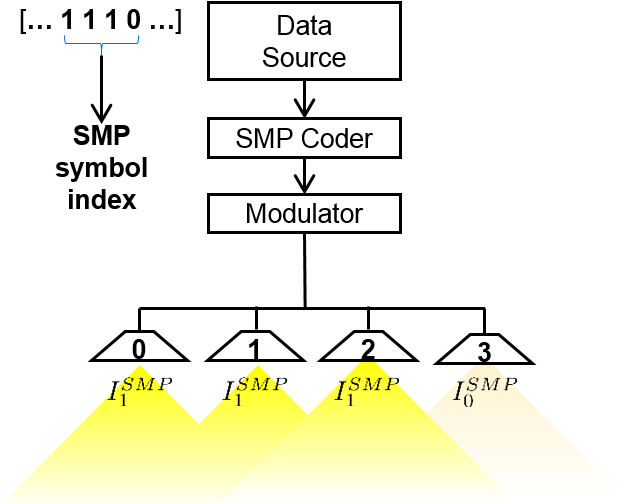
\includegraphics[trim=0in 0in 0in 0in, clip=false, width=2.5in]{figSMP.png}
				\caption{}
				\label{figSMP}
		\end{subfigure}
\caption{Illustration of (a) SM operation with $N_{\text{tx}} = 4$ and $M = 4$. (b) SMP operation with $N_{\text{tx}} = 4$ and $M = 2$.}
	\label{fig:SpatialModulation}
\end{figure}

Optical spatial modulation (SM) was introduced in \cite{mes06a} as a low complexity modulation technique that enhances spectral efficiency by exploiting spatial dimension. SM encodes $k =$ log$^{ }_{2}(N_{\text{tx}})$ bits in the transmitter index in addition to $m=$ log$^{ }_{2}(M)$ bits using $M$-ary modulation. Thus SM transmits $r=k+m=$ log$^{ }_{2}(MN_{\text{tx}})$ bits per SM symbol. The encoded information stream is divided into $r$ bits long contiguous segments. First $m$ bits of each symbol are mapped to one of the $M$-ary constellation points while the last $k$ bits of each symbol select the luminaire that transmits the selected constellation point. SM implementation is illustrated in \figurename{ \ref{figSM}} for $N_{\text{tx}}=4$ transmitters and 4-PAM. $M$-PAM intensity levels for SM are selected as in (\ref{eqSMPAM}) where $P^{\text{tx}}_{\text{avg}}$ is the average signal constraint to maintain desired illumination. Given a bit sequence forming a symbol [1 1 1 0], PAM level 3 $(I_4^{\text{SM}})$ is radiated using transmitter index $2$.

\begin{equation}
	\label{eqSMPAM}
	P_{x}^{\text{SM}} = \frac{2P^{\text{tx}}_{\text{avg}}}{M+1}x; 1 \leq x \leq M
\end{equation}

On the other hand, spatial multiplexing (SMP) uses $M$-ary modulation for each luminaire to transmit information. In SMP with $N_{\text{tx}}$ number of luminaires jointly generates $M^{N_{\text{tx}}}$ unique symbols. Each SMP symbols transmits $r=N_{\text{tx}}$ log$^{ }_{2}(M)$ bits. Each $r$ bit long section of encoded information stream is then mapped to one of the $M^{N_{\text{tx}}}$ unique symbols. SMP for a setup with $N_{\text{tx}}=4$ transmitters and 2-PAM is illustrated in \figurename{ \ref{figSMP}}. $M$-PAM intensity levels for SMP are selected as in (\ref{eqSMPPAM}) where $P^{\text{tx}}_{\text{avg}}$ is the average signal constraint to maintain desired illumination. A bit sequence forming a symbol [1 1 1 0] is jointly mapped to the $15^{th}$ out of $N_{\text{tx}}$log$^{ }_{2}(M)=16$ possible unique symbols.
\begin{equation}
	\label{eqSMPPAM}
	P_{x}^{\text{SMP}} = \frac{2P^{\text{tx}}_{\text{avg}}}{M-1}x; 0\leq x < M
\end{equation}

For a channel with equally likely symbols, a maximum likelihood detector is the optimal detector. If noise is AWGN, this reduces to nearest neighbor detection. Having observed ${\bf{Y}}$ and knowing ${\bf{H}}$, estimated symbol $\hat{{\bf{X}}}$ is the symbol closest to observation ${\bf{Y}}$ in Euclidean space. The signal detection can be written as
\begin{gather}
\begin{aligned}
	\hat{{\bf{X}}} =&{} \argmax_{\forall{\bf{X_i}}} p_{{\bf{Y}}|{\bf{X}}}({\bf{Y}}|{\bf{X_i}},{\bf{H}})\\
	=&{} \argmin_{\forall{\bf{X_i}}} ||{\bf{Y}}-{\bf{H}}{\bf{X_i}}||_{F}
\label{eq:ML}
\end{aligned}
\end{gather}
where ${\bf{X_i}}$ are the different symbols and $||.||_{F}$ is the Frobenius norm.

In an indoor VLC system, luminaires need to maintain an average emitted radiant flux over different overlapping time windows so that the perceived illumination remains constant. Thus a fair performance comparison between different modulation schemes can be made when they emit the same radiant flux. Thus the SNR is defined as
\begin{equation}
  \label{eqOSMSNRTX}
	\text{SNR} = \frac{(\text{e}P_{\text{avg}}^{\text{tx}})^2}{\sigma_{n}^2}
\end{equation}
where $P_{\text{avg}}^{\text{tx}}$ is the average radiant flux emitted by a transmitter, e is the optical to electrical conversion factor (AW$^{-1}\Omega^{-2})$ and $\sigma_{n}^2$ is the noise power. Without loss of generality, e = 1 is assumed. This is similar definition as in \cite{fat13a} and is used to demonstrate performance enhancement of SM and SMP systems with imaging receiver when compared to non--imaging receiver considered in the reference.
%%%%%%%%%%%%%%%%%%%%%%%%%%%%%%%%%%%%%%%%%%%%%%%%%%%%%%%%%%%%%%%%
%%%%%%%%%%%%%%%%%%%%%%%%%%%% RESULTS %%%%%%%%%%%%%%%%%%%%%%%%%%%
%%%%%%%%%%%%%%%%%%%%%%%%%%%%%%%%%%%%%%%%%%%%%%%%%%%%%%%%%%%%%%%%

\subsection{Performance with imaging receiver}
\label{subsec:osmAnalysis}
% DELETED ON 11 MARCH 2015
%An example system is considered which has 4 transmitters arranged on a regular grid with pitch $P_{\text{tx}}$. Each transmitter has side length $\alpha_{\text{tx}}^{min}$ and diagonal $\alpha_{\text{tx}}^{max}$. The imaging receiver optics has focal length $f$. Sensor is made of large enough contiguous PD array such that all the 4 transmitter images (spots) fall on the sensor for all the different analysis configurations. Each PD is assumed to have a square shape with side length $\alpha_{\text{px}}^{min}$ and diagonal $\alpha_{\text{px}}^{max}$. The receiver surface is assumed parallel to the transmitter plane. Receiver at a distance $d$ from the transmitter plane sees a magnification $M=f/(d-f)$. If $d>>f$, which is true is most practical scenarios, $M\approx f/d$. 

The effects of varying transmitter array and imaging receiver configurations on the BER performance of SM and SMP systems are studied. An array of $N_{\text{tx}} = 4$ transmitters that are arranged on a regular grid with pitch $P_{\text{tx}}$ is considered. To achieve 4 bits/sym, SM with $N_{\text{tx}}=4$ and $M=4$-PAM and SMP with $N_{\text{tx}}=4$ and $M=2$-PAM are implemented. To achieve 8 bits/sym, SM with $N_{\text{tx}}=4$ and $M=64$-PAM and SMP with $N_{\text{tx}}=4$ and $M=4$-PAM are implemented. The vertical distance $||\vm{d}^{z}_{j}||$ between the transmitter and receiver planes is 2 m. Lambertian luminaires of order 1 are assumed to have a spectral power distribution that is approximated by a sum of Gaussians as in \cite{gru08b}. The effective responsivity of each pixel is equal to 0.4 A/W. Within this context, it is assumed that the pixel grid is large enough to ensure that each of the four spots fall on the sensor for each of the different configurations considered below.

Using the parameters specified above, the channel gains are of the order of $10^{-7}$ for all configurations. Thus the transmitted signal power is about $140$dB higher than the received signal power. Typically, the SNR is defined as the ratio of received signal power to noise power. However, given SNR as defined in Eq. \eqref{eqOSMSNRTX}, there is an offset of at least +140 dB over typical definition.

%%%%%%%%%%%%%%%%%%%%%%%%%%%%%%%%%%%%%%%%%%%
%%%%%%%%%%%%%%%%% COMPARE %%%%%%%%%%%%%%%%%
%%%%%%%%%%%%%%%%%%%%%%%%%%%%%%%%%%%%%%%%%%%
\subsubsection{Imaging vs non--imaging receiver}
\label{subsubsec:osmResultsCompare}
Performance gains of using an imaging receiver over a non--imaging receiver are analyzed in this subsection. The transmitter and modulation parameters are the same as described above. For this analysis, $P_{\text{tx}}=$ 0.5 m is considered. The non--imaging receiver is made up of $2\times2$ array of pixels; each with a side length of 1 mm and a pitch of 1 mm. Each pixel has a concentrator of refractive index $1.5$ and field-of-view (FOV) of 60 $\deg$. For the imaging receiver, the sensor is modeled as $2\times2$ array of pixels with side length and pitch of 1 mm. The imaging lens is defined to have sufficient magnification to align the images of the four transmitters each with four pixels respectively. 
\afterpage{%
	\clearpage
\begin{figure}
	\centering
		\begin{subfigure}{\textwidth}
			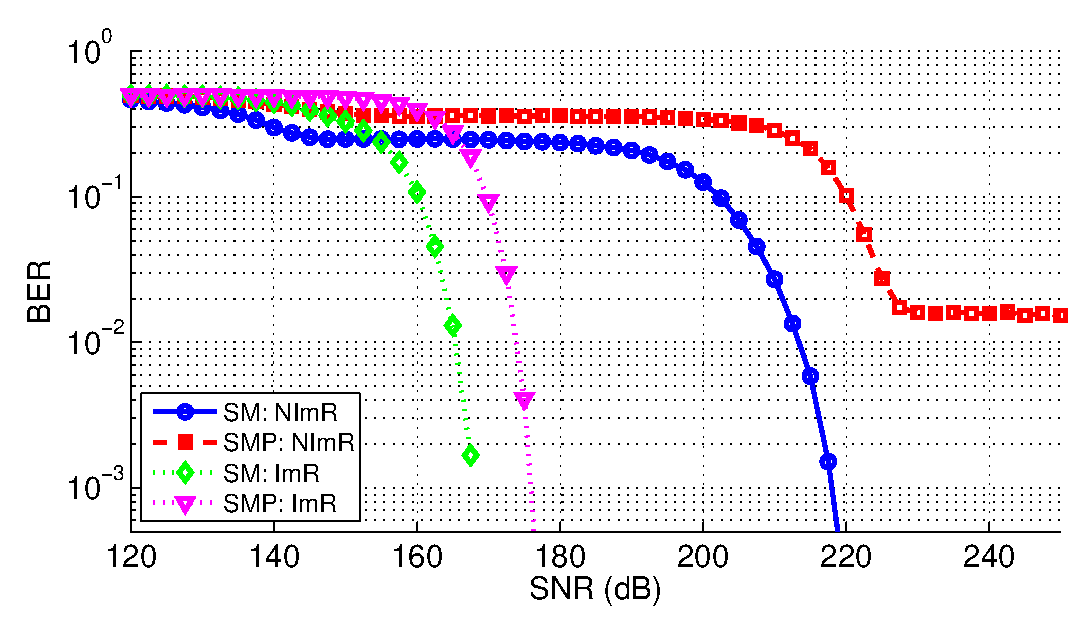
\includegraphics[width=0.9\textwidth]{figCompare4B.eps}
			\caption{4 bits/sym}
			\label{figCompare4B}
		\end{subfigure}
	  \vfill
		\begin{subfigure}{\textwidth}
		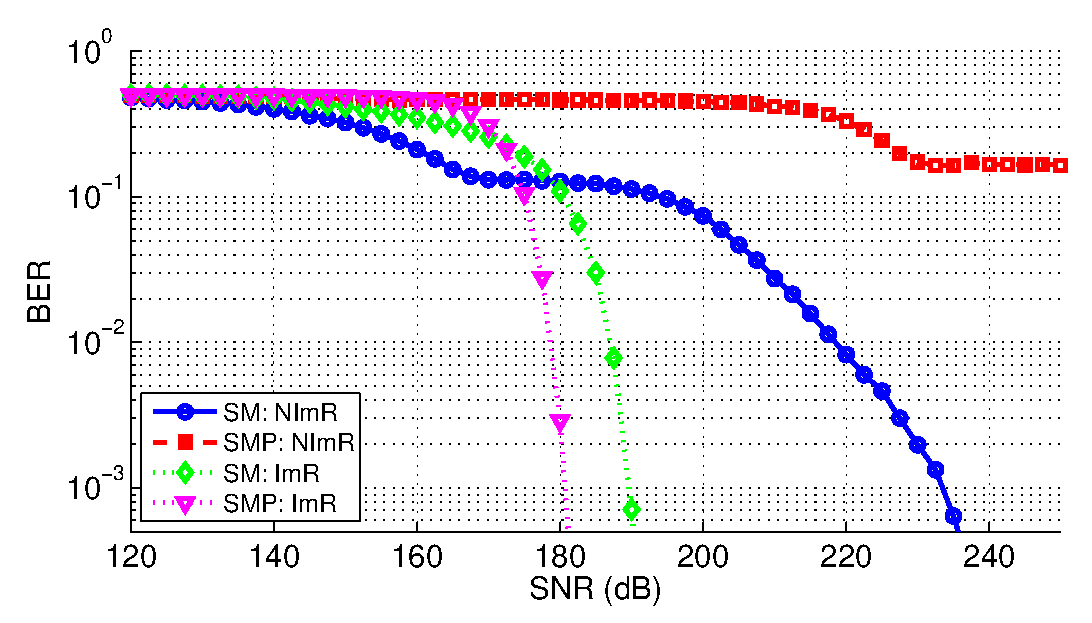
\includegraphics[width=0.9\textwidth]{figCompare8B.eps}
		\caption{8 bits/sym}
		\label{figCompare8B}
		\end{subfigure}
	
	\caption{Performance comparison of SM and SMP using non--imaging (NImR) and imaging (ImR) receiver}
	\label{figCompare}
\end{figure}
\clearpage% Flush page
}
The FOV of the receiver changes with the sensor dimensions. The maximum FOV is defined as 60 $\deg$; the same as in non--imaging receiver case. A fair performance comparison between the two receiver configurations can be made under the assumption that the same average signal radiant flux is incident on both. Thus, the aperture of the imaging receiver is modeled to have an area of  1 mm$^{2}$.

BER vs SNR curves for SM and SMP using non--imaging receiver and imaging receiver are shown in \figurename{ \ref{figCompare}}. At low average signal powers, using a non--imaging receiver, shot noise is the dominant source of noise. At high signal powers, ICI dominates the noise for the non--imaging receiver because the channel matrix coefficients are highly correlated \cite{zen09a}. This can be seen as two regions of the BER curves when using a non--imaging receiver. SM mitigates ICI and is thus more robust as compared to SMP in this scenario. BER achieved by SMP with non--imaging receiver are greater than $10^{-3}$ for the range of SNR considered and thus cannot be improved by forward error correction (FEC). SM needs a high transmit signal power to achieve BER$=10^{-3}$ for both 4 and 8 bits/sym. Conversely, imaging receiver completely demultiplexes the four transmit signals while generating a diagonal channel matrix and thus avoids ICI under ideal setup. To achieve BER $=10^{-3}$ at 4 bits/sym, SM with imaging receiver performs about 8 dB better that SMP with imaging receiver and about 45 dB better than SM with non--imaging receiver. SMP packs more bits spatially in transmitter location as compared to SM. Thus, to achieve higher spectral efficiency while keeping the number of transmitters the same, more $M$-ary PAM levels are needed for SM as compared to SMP thus quickly degrading SM's performance. To achieve BER $=10^{-3}$ at 8 bits/sym, SMP with imaging receiver outperforms SM with imaging receiver by about 10 dB and SM with non--imaging receiver by about 52 dB. The channel matrix coefficient decorrelation afforded by imaging receiver provide huge SNR gains over non--imaging receiver for a given BER.

%%%%%%%%%%%%%%%%%%%%%%%%%%%%%%%%%%%%%%%%%%%%
%%%%%%%%%%%%%%%%%%% ALPHA %%%%%%%%%%%%%%%%%%
%%%%%%%%%%%%%%%%%%%%%%%%%%%%%%%%%%%%%%%%%%%%

\subsubsection{Varying $\alpha_{s}$}
\label{subsec:osmResultsAlpha}

\begin{figure}[!t]
	\centering
		\begin{subfigure}{0.49\textwidth}
			\centering
			\includegraphics[width=0.65\textwidth]{figASspN4A05.eps}
			\label{figASspN4A05}
		\caption{$\alpha_{s}=0.5$}
		\end{subfigure}
		\hfill
		\begin{subfigure}{0.49\textwidth}
			\centering
			\includegraphics[width=0.65\textwidth]{figASspN4A1.eps}
			\label{figASspN4A1}
		\caption{$\alpha_{s}=1.0$}
		\end{subfigure}
		\vfill
		\begin{subfigure}{0.49\textwidth}
			\centering
			\includegraphics[width=0.65\textwidth]{figASspN4A14.eps}
			\label{figASspN4A14}
		\caption{$\alpha_{s}=1.41$}
		\end{subfigure}
		\hfill
		\begin{subfigure}{0.49\textwidth}
			\centering
			\includegraphics[width=0.65\textwidth]{figASspN4A2.eps}
			\label{figASspN4A2}
		\caption{$\alpha_{s}=2.0$}
		\end{subfigure}
	\caption{Spots on the sensor for different $\alpha_{s}$}
	\label{figASSpots}
\end{figure}

\afterpage{%
	\clearpage
\begin{figure}
	\centering
		\begin{subfigure}{\textwidth}
			\centering
			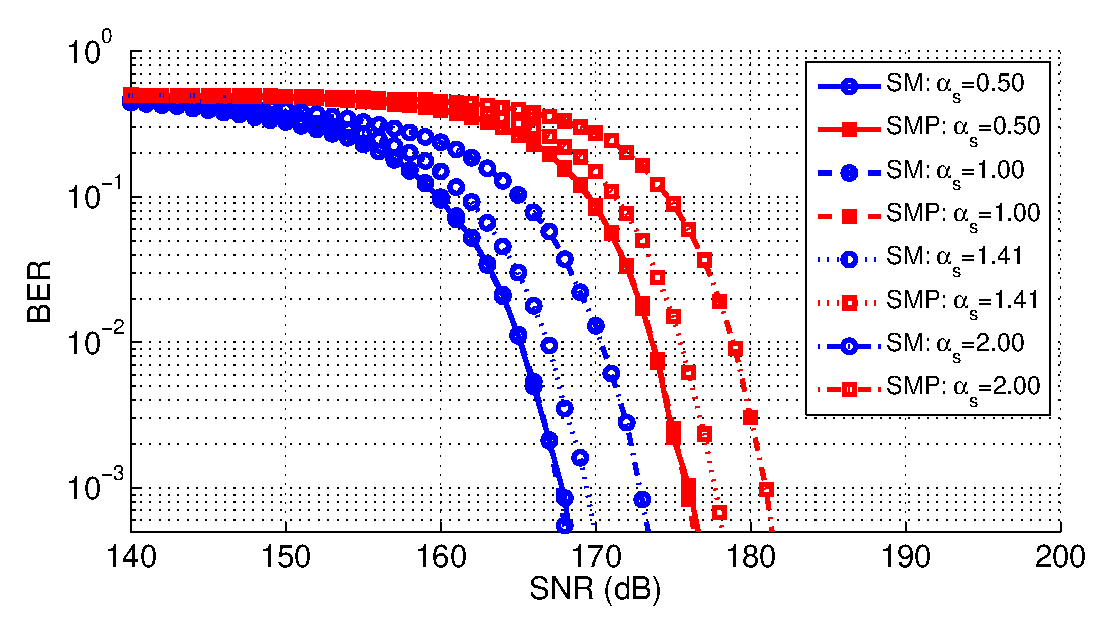
\includegraphics[width=0.9\textwidth]{figASN4B4.eps}
			\caption{4 bits/sym}
			\label{figASN4B4}
		\end{subfigure}
		
		\begin{subfigure}{\textwidth}
			\centering
			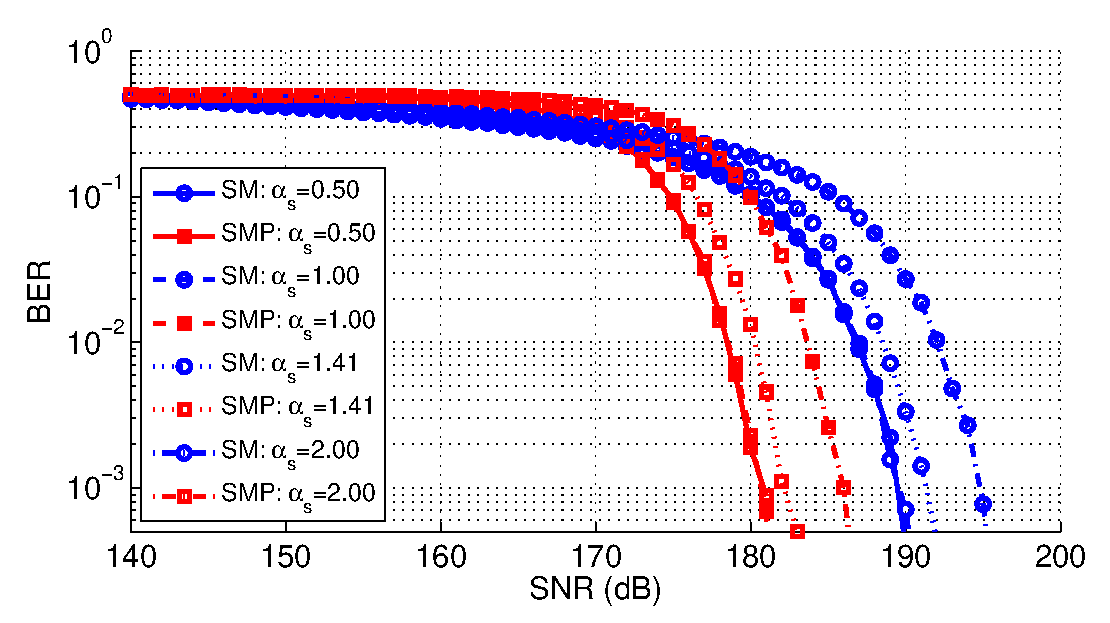
\includegraphics[width=0.9\textwidth]{figASN4B8.eps}
			\caption{8 bits/sym}
			\label{figASN4B8}
		\end{subfigure}
		
		\caption{BER vs SNR for different $\alpha_{s}$}
		\label{figASBvS}
\end{figure}
	\clearpage% Flush page
}

For this analysis, $\alpha_{s}$ is varied while keeping $\delta_{s}$ and $\mu_{s}$ fixed. As illustrated in \figurename{ \ref{figASSpots}}, $\alpha_{s}$ affects only the spot size. As $\alpha_{s}$ increases, spots on the sensor overlap increasingly more number of pixels degrading the BER performance. Increasing the number or pixels per spot also increases the noise for each link thus causing the drop in performance. Very small pixel sizes or very large transmitter sizes also cause increase in $\alpha_{s}$. A smaller pixel size does enable the system to pack more channels provided $\alpha_{s}$ is relatively small. On the other hand, having very small pixel sizes or alternately large transmitter illumination surface tend to increase $\alpha_{s}$ and force the system to operate in a suboptimal configuration.

BER vs SNR curves for SM and SMP for different values of $\alpha_{s}$ are shown in \figurename{ \ref{figASBvS}}. To achieve BER $\leq10^{-3}$ at 4 bits/sym, SNRs of about [168, 168, 170, 173]dB and [176, 176, 178, 181] dB are needed for $\alpha_{s}$ = [0.5, 1, 1.41, 2]  with SM and SMP respectively. To achieve BER $\leq10^{-3}$ at 8 bits/sym, SNRs of about [190, 190, 192, 195] dB and [181, 181, 183, 186] dB are needed for $\alpha_{s}$ = [0.5, 1, 1.41, 2] with SM and SMP respectively. Thus there is about a 2 dB SNR penalty for system operating at $\alpha_{s}=1.41$ and 5 dB SNR penalty for system operating at $\alpha_{s}=2$ as compared to that at $\alpha_{s}=1$.

%%%%%%%%%%%%%%%%%%%%%%%%%%%%%%%%%%%%%%%%%%
%%%%%%%%%%%%%%%%%%% ETA %%%%%%%%%%%%%%%%%%
%%%%%%%%%%%%%%%%%%%%%%%%%%%%%%%%%%%%%%%%%%
\subsubsection{Varying $\eta_{s}$}
\label{subsubsec:osmResultsEta}
\begin{figure}[!t]
	\centering
		\begin{subfigure}{0.49\textwidth}
			\centering
			\includegraphics[width=0.65\textwidth]{figESspN4E0.eps}
			\caption{$\eta_{s}=0$}
			\label{figESspN4E0}
		\end{subfigure}
		\hfill
		\begin{subfigure}{0.49\textwidth}
			\centering
			\includegraphics[width=0.65\textwidth]{figESspN4E071.eps}
			\caption{$\eta_{s}=0.71$}
			\label{figESspN4E071}
		\end{subfigure}
		\vfill
		\begin{subfigure}{0.49\textwidth}
			\centering
			\includegraphics[width=0.65\textwidth]{figESspN4E1.eps}
			\caption{$\eta_{s}=1$}
			\label{figESspN4E1}
		\end{subfigure}
		\hfill
		\begin{subfigure}{0.49\textwidth}
			\centering
			\includegraphics[width=0.65\textwidth]{figESspN4E14.eps}
			\caption{$\eta_{s}=1.41$}
			\label{figESspN4E14}
		\end{subfigure}
		
		\caption{Spots on sensor for different $\eta_{s}$}
		\label{figESSpots}
\end{figure}

For this analysis, $\eta_{s}$ (alternately $\delta_{s}$) is varied while keeping $\alpha_{s}$ and $\mu_{s}$ fixed. Thus only the effect of change in spot pitch affects the BER performance. As illustrated in \figurename{ \ref{figESSpots}}, as $\eta_{s}$ increases, distance between the spots on the sensor increases as they push further apart.

\afterpage{%
	%\clearpage
	\begin{figure}
		\centering
			\begin{subfigure}{\textwidth}
				\centering
				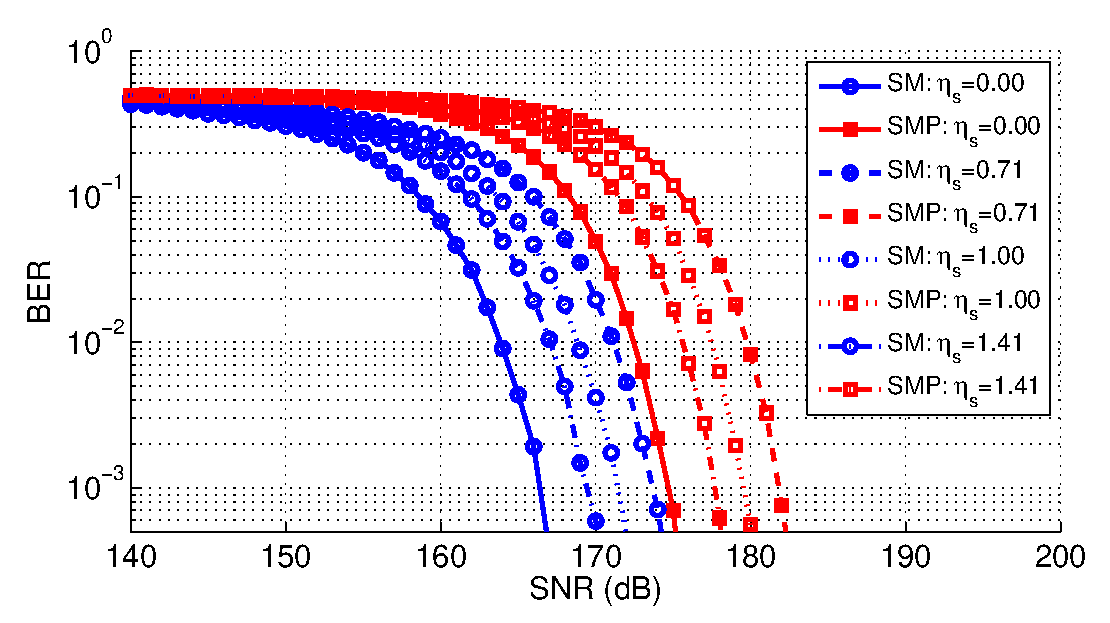
\includegraphics[width=0.9\textwidth]{figESN4B4.eps}
				\caption{4 bits/sym}
				\label{figESN4B4}
			\end{subfigure}
			\vfill
			\begin{subfigure}{\textwidth}
				\centering
				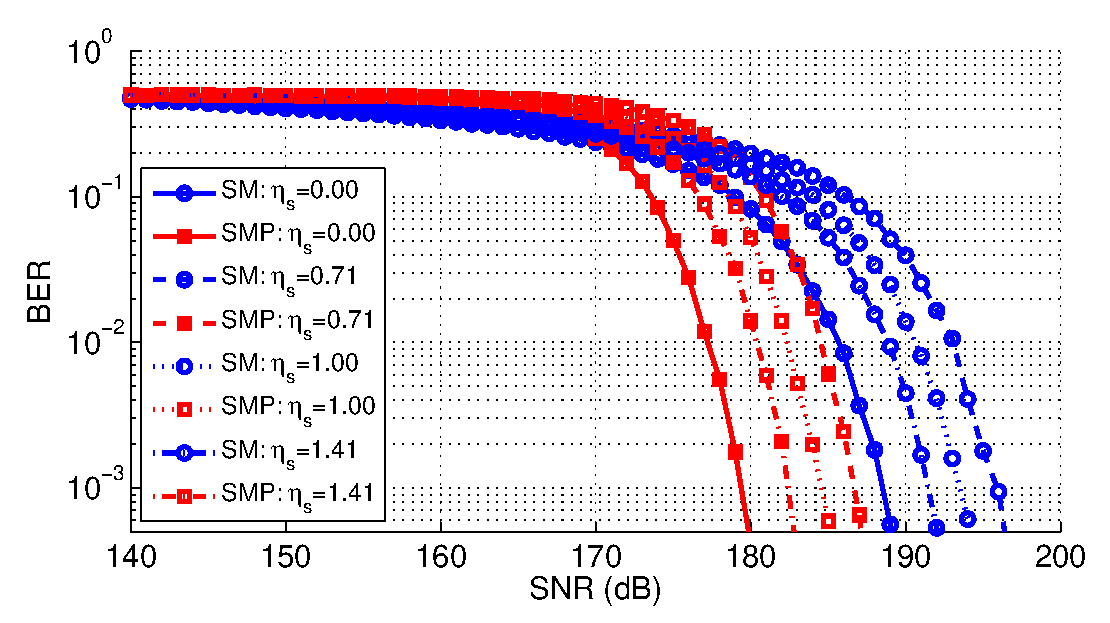
\includegraphics[width=0.9\textwidth]{figESN4B8.eps}
				\caption{8 bits/sym}
				\label{figESN4B8}
			\end{subfigure}
			
			\caption{BER vs SNR for different $\eta_{s}$.}
			\label{figESBvS}
	\end{figure}
	%\clearpage% Flush page
}
BER vs SNR curves for SM and SMP for different values of $\eta_{s}$ are shown in \figurename{ \ref{figESBvS}}. To achieve BER $\leq 10^{-3}$ at 4 bits/sym, SNRs of about [167, 174, 172, 170] dB and [175, 182, 180, 178] dB are needed for $\eta_{s}$ = [0, 0.71, 1, 1.41] with SM and SMP respectively. To achieve BER $\leq 10^{-3}$ at 8 bits/sym, SNRs of about [189, 196, 194, 192] dB and [180, 187, 185, 183] dB are needed for $\eta_{s}$ = [0, 0.71, 1, 1.41] with SM and SMP respectively. We see that the BER performance is best when the spot overlaps minimum number of pixels and worst when the spot is centered at a corner of a pixel thus maximizing the number of pixels it overlaps with. In this setup, for BER $=10^{-3}$, there is an SNR penalty of about 7 dB between the best and worst cases. The slight drop in performance for $\eta_{s}=1.4$ as compared to $\eta_{s}=0$ can be attributed to drop in free-space gain caused by the larger distance per link longer as a result of increased transmitter pitch.

%%%%%%%%%%%%%%%%%%%%%%%%%%%%%%%%%%%%%%%%
%%%%%%%%%%%%%%%%%% MU %%%%%%%%%%%%%%%%%%
%%%%%%%%%%%%%%%%%%%%%%%%%%%%%%%%%%%%%%%%
\subsubsection{Varying $\mu_{s}$}
\label{subsubsec:osmResultsMu}
\begin{figure}[!t]
	\centering
		\begin{subfigure}{0.49\textwidth}
			\centering
			\includegraphics[width=0.65\textwidth]{figMSspN4M05.eps}
			\caption{$\mu_{s}=0.5$}
			\label{figMSspN4M05}
		\end{subfigure}
		\hfill
		\begin{subfigure}{0.49\textwidth}
			\centering
			\includegraphics[width=0.65\textwidth]{figMSspN4M1.eps}
			\caption{$\mu_{s}=1$}
			\label{figMSspN4M1}
		\end{subfigure}
		\vfill
		\begin{subfigure}{0.49\textwidth}
			\centering
			\includegraphics[width=0.65\textwidth]{figMSspN4M14.eps}
			\caption{$\mu_{s}=1.41$}
			\label{figMSspN4M14}
		\end{subfigure}
		\hfill
		\begin{subfigure}{0.49\textwidth}
			\centering
		\includegraphics[width=0.65\textwidth]{figMSspN4M2.eps}
			\caption{$\mu_{s}=2$}
			\label{figMSspN4M2}
		\end{subfigure}
		\caption{Spots on sensor for different $\mu_{s}$}
		\label{figMSSpots}
\end{figure}

\afterpage{%
	%\clearpage
	\begin{figure}
		\centering
			\begin{subfigure}{\textwidth}
				\centering
				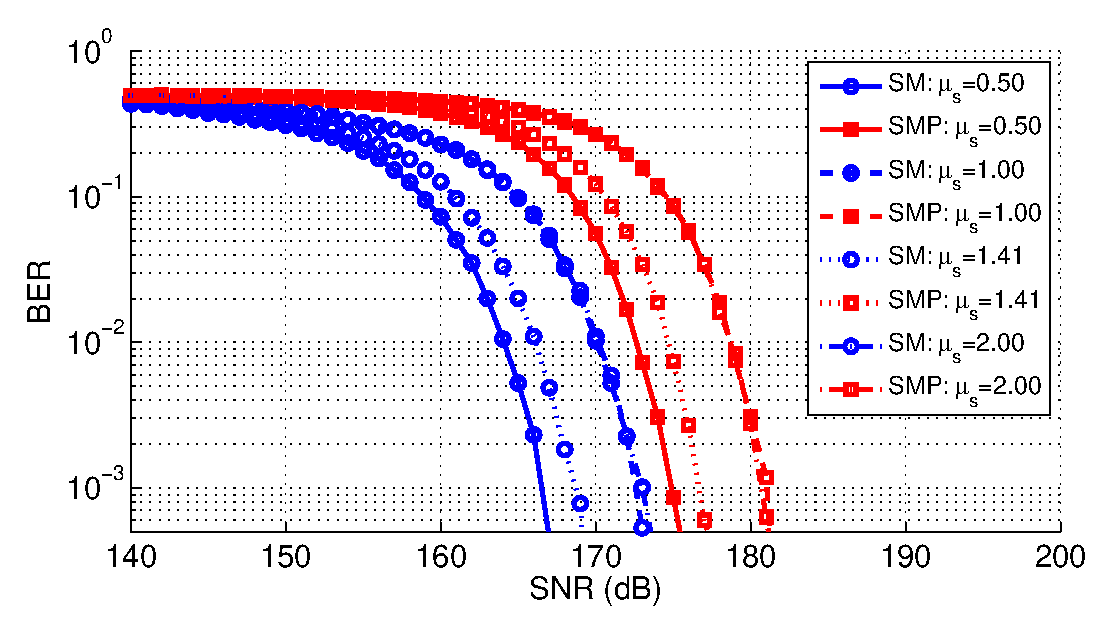
\includegraphics[width=0.9\textwidth]{figMSN4B4.eps}
				\caption{4 bits/sym}
				\label{figMSN4B4}
			\end{subfigure}
			
			\begin{subfigure}{\textwidth}
				\centering
				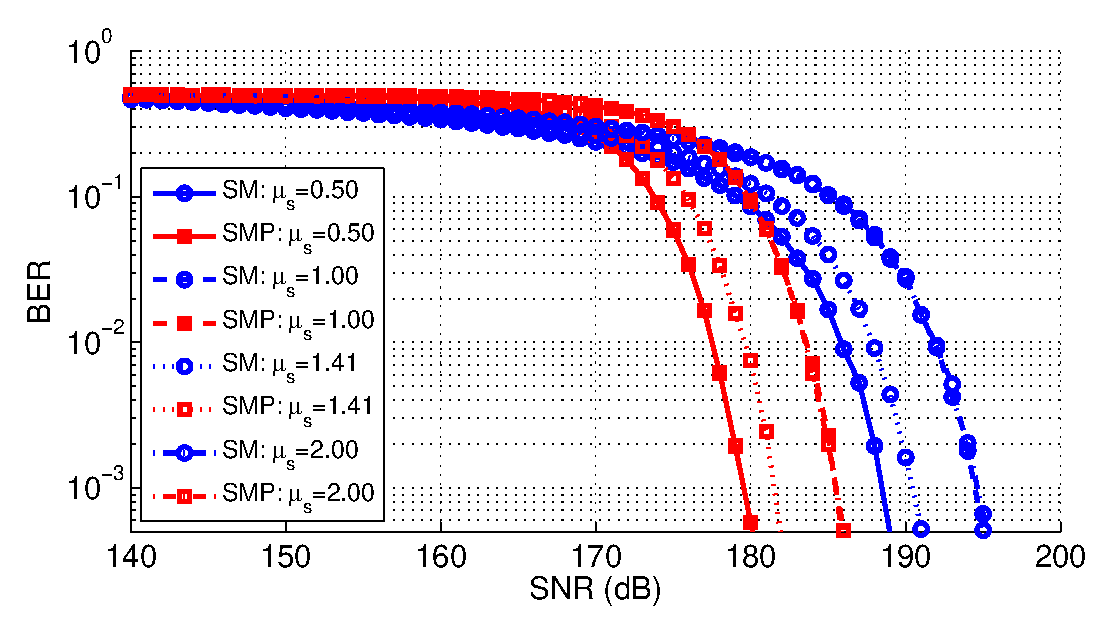
\includegraphics[width=0.9\textwidth]{figMSN4B8.eps}
				\caption{8 bits/sym}
				\label{figMSN4B8}
			\end{subfigure}
			
			\caption{BER vs SNR for different $\mu_{s}$}
			\label{figMSBvS}
	\end{figure}
	%\clearpage% Flush page
}

In this analysis, $\mu_{s}$ is varied by varying $f$. Alternately, it can be varied by changing $||\vm{d}^{z}_{j}||$. Varying $\mu_{s}$ affects both $\alpha_{s}$ and $\eta_{s}$ simultaneously. This captures their combined impact on the BER performance. We see from \figurename{ \ref{figMSSpots}} that increasing $\mu_{s}$ not only increases the spot size but also pushes the spots away from each other. Note unlike in previous case, the transmitter pitch remains constant ($P_{\text{tx}}>0$).

BER vs SNR curves for SM and SMP for different values of $\mu_{s}$ are shown in \figurename{ \ref{figMSBvS}}. To achieve BER $=10^{-3}$ at 4 bits/sym, SNRs of about [167, 173, 169, 173] dB and [175, 181, 177, 181]dB are needed for $\mu_{s}$ = [0.5, 1, 1.41, 2] with SM and SMP respectively. To achieve BER $=10^{-3}$ at 8 bits/sym, SNRs of about [189, 195, 191, 195] dB and [180, 186, 182, 186] dB are needed for $\mu_{s}$ = [0.5, 1, 1.41, 2] with SM and SMP respectively.

The best performance is obtained for $\mu_{s}\leq 0.5$. This is because at this value of $\mu_{s}$, $\alpha_{s}<1$ and $\eta_{s}$ is such that all spots lie on different adjacent pixels. It can also be inferred that given enough transmitters in the room, at $\mu=0.5$, every single pixel could get signal from a single transmitter thus greatly improving the capacity of the channel. If the luminaires transmit with different power levels or if the channels gains are significantly different, capacity maximizing $\mu_{s}$ is an optimization problem to be solved.

At lower bit rates, SM benefits from having higher transmit power per symbol at lower $M$-PAM level. To achieve higher bit-rates, higher $M$-PAM levels push the constellations closer to each other thus quickly degrading the SM performance as compared to SMP. As shown in \figurename{ \ref{figASBvS}}, \figurename{ \ref{figESBvS}} and \figurename{ \ref{figMSBvS}}, to achieve BER $=10^{-3}$, at 4 bits/sym, SM performs 8-10 dB better while at 8 bits/sym, SMP performs 8-10 dB better.


%\begin{figure}
	%\centering
		%\begin{subfigure}{\textwidth}
			%\caption{}
			%\label{}
		%\end{subfigure}
		%\caption{}
		%\label{}
%\end{figure}

% -------------------------------------
% SECTION: SIS-OFDM
% -------------------------------------
\section{Sample Indexed Spatial Orthogonal Frequency Division Multiplexing}
\label{sec:sisofdm}

\graphicspath{{_MIMOSpace/figures_sisofdm/}}

Recently, the increase in use of portable computing devices has created an intense demand for wireless data access. Spectral allocations and regulations limit our ability to increase the capacity of existing channels within the radio frequency (RF) spectrum. Advances made in the solid-state lighting industry are driving significant deployments of energy-efficient light emitting diode (LED) based luminaries. This has created an opportunity to use such luminaries to establish high capacity indoor visible light communication (VLC) links and reduce the bottleneck on existing RF wireless channels. Under this model, luminaries simultaneously support illumination and wireless data transmission \cite{elg11a}. OSM and O-OFDM are two techniques that have been proposed to implement such a dual-use VLC channel.

OSM is a multiple-transmitter technique in which information is encoded over (a) index of luminiares that are spatially separated and (b) modulation scheme overlayed on indexed luminaire \cite{mes10a}. Within a symbol period, only one luminaire emits a radiant flux while all other luminaires are idle. This minimizes the inter-channel interference (ICI) thus simplifying the detection process and the overall system complexity as compared to spatial multiplexing (SMP). In OSM, the bit-stream to be transmitted is divided into contiguous sections of $k=log_2(N_{tx})$ spatial bit-stream and $m=log_2(M)$ modulation bit-stream where $N_{tx}$ is the number of luminaires and $M$ is the modulation order. The $k$ bits select the luminaire to be activated while the $m$ bits select the M-ary modulation symbol to be transmitted. Thus, OSM system provides $log_2(MN_{tx})$ bits per symbol. In \cite{fat11a}, an OSM system with pulse amplitude modulation (PAM) as the overlayed modulation scheme is proposed. Reference \cite{pop12a} proposes a scheme that combines OSM with pulse position modulation (PPM) to benefit from the energy efficiency of PPM as compared to PAM. Reference \cite{but14a} shows ImR can provide significant SNR gains for OSM and SMP as compared to NImR.

\afterpage{%
	\clearpage
	\begin{landscape}% Landscape page
		\begin{figure}[!t]
			\centering
			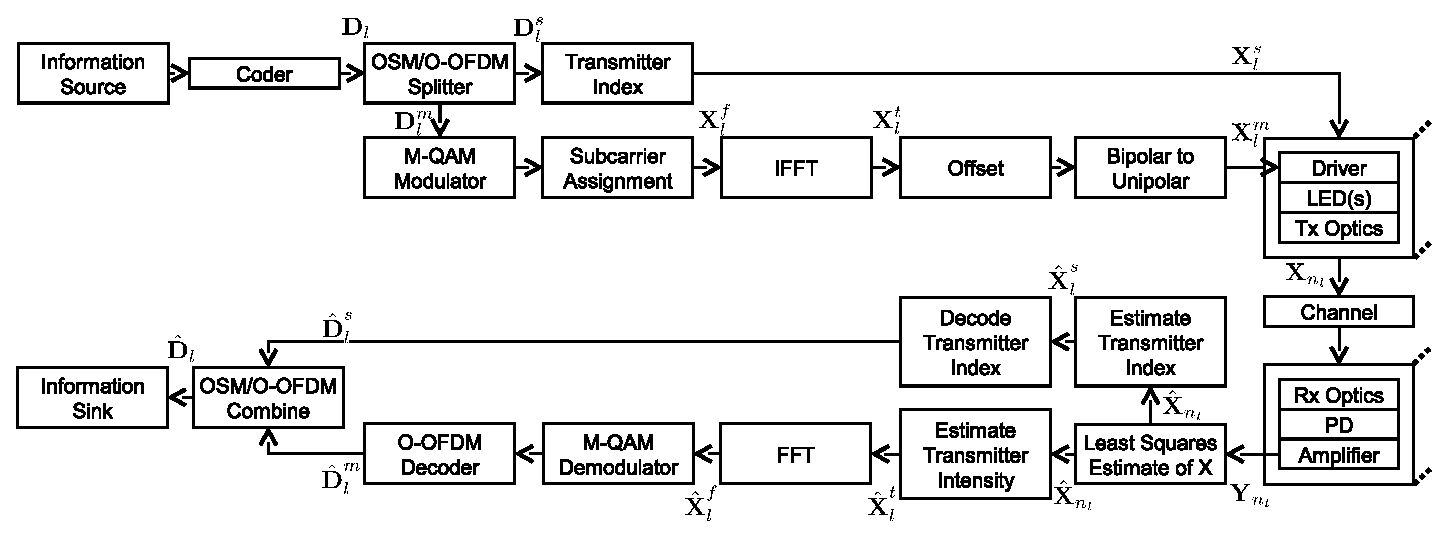
\includegraphics[trim={0.0in 0.0in 0.0in 0.0in}, clip=false, width=1.3\textwidth]{figBlockDiagram2.eps}
			\caption{Block diagram of system implementing SIS-OFDM}
			\label{figBlockDiagram}
		\end{figure}
	\end{landscape}
	\clearpage% Flush page
}

Implementation and performance comparisons of ACO-OFDM and DCO-OFDM is shown in reference \cite{mes11a}. In ACO-OFDM, data is assigned only on odd subcarriers while in DCO-OFDM all odd and even subcarriers are assigned data. Hermetian symmetry is enforced across the frequency-domain O-OFDM symbol. An inverse fast fourier transform (IFFT) process then results in a real-valued time domain signal that multiplexes the streams before transmission over the channel. In IM/DD systems, the signal is transmitted by varying the output flux from the transmitter. Thus, the transmitted signal must be non-negative and real valued. The ACO-OFDM signal can be clipped at values below zero because the resulting clipping noise is shown to be orthogonal to the signal \cite{arm06a}. Conversely, in DCO-OFDM an offset must be added to the multiplexed signal in order to minimize errors due to clipping of negative valued signal. O-OFDM achieves high spectral efficiency by enabling parallel transmission of higher order modulation symbols on orthogonal subcarriers. The number of data-subcarriers, $N_{sc}^d$, equals ($N_{sc}/4$) for ACO-OFDM and ($N_{sc}/2-1$) for DCO-OFDM where $N_{sc}$ is the total number of subcarriers. Thus the number of transmitted bits per O-OFDM symbol is given by $R^{m}=N_{sc}^d\times log_2(M)$.

An approach to combine OSM and traditional OFDM is proposed in reference \cite{gan06a}. This approach is adapted for IM/DD communications in reference \cite{zha12a}. Here, an incoming bit-stream is divided into O-OFDM and OSM streams. Data from O-OFDM stream is assigned to different subcarriers to form the frequency domain O-OFDM symbol. OSM is then implemented in the frequency domain where each data-subcarrier is assigned to a transmitter determined by the spatial bit-stream. An IFFT operation is implemented at each transmitter to multiplex the data before transmission. Spectral efficiency of this scheme is then proportional to the number of data-subcarriers. In comparison, the spectral efficiency of SIS-OFDM is proportional to the number of subcarriers which is equal to at least double the number of data-subcarriers. Additionally, the SIS-OFDM system requires a single IFFT operation, independent of the number of transmitters and thus maintains a computational complexity equal to that of SISO OFDM transmission. Finally, SIS-OFDM using an ImR achieves much better power efficiency as compared to equivalent system using NImR.

\figurename{\ref{figBlockDiagram}} illustrates the block diagram of a system implementing SIS-OFDM. The information source generates the input data-stream. The coder converts the data-stream into a binary bit-stream $\vm{D}$ which is divided into consecutive segments of $R^{ms}=R^{m}+R^{s}$ bits where $R^{s}=N_{sc}\times k=N_{sc}\times log_2(N_{tx})$ is the number of spatial bits . Let the $l^{th}$ such segment be denoted by $\vm{D}_l$. The first $R^{m}$ bits of $\vm{D}_l$ are collected in a vector $\vm{D}_l^m$ are are mapped by an M-QAM modulator. The generated QAM symbols are then assigned to subcarriers (based on the O-OFDM signal format, \textit{i.e.} DCO-OFDM or ACO-OFDM) to generate a frequency-domain O-OFDM symbol $\vm{X}_l^f$ of length $N_{sc}$. An IFFT operation is applied on $\vm{X}_l^f$ to produce a real-valued bipolar time-domain O-OFDM symbol $\vm{X}_l^t$ of the same length $N_{sc}$. The latter $R^{s}$ bits of $\vm{D}_l$ are collected in a vector $D_l^s$ and are mapped to $N_{sc}$ length transmitter index vector denoted by $\vm{X}_l^s$. Let $\vm{X}_l^m$ denote the real unipolar baseband signal after biasing and/or clipping, and $0\leq n_l\leq (N_{sc}-1)$ indicate the relative time index for the next SIS-OFDM symbol to be transmitted. At each time instance, an O-OFDM signal value from $\vm{X}_l^m$ is transmitted from a luminaire indexed by $\vm{X}_l^s$. Let $\vm{X}_{n_l}$ be this $N_{tx}$ length transmission vector at time instant $n_l$. Thus the $j^{th}$ element of this vector is then given by
\begin{equation}
	\label{eqX}
	\vm{X}_{n_l}(j) = \twopartdef{\vm{X}_l^m(n_l)}{j=\vm{X}_l^s(n_l)}{0}{\text{else}}
\end{equation}

The SIS-OFDM symbol and transmit vector generation is explained using the following example which considers ACO-OFDM with $N_{sc}=8$, 4-QAM subcarrier modulation and $N_{tx}=2$. Here, $R^{m}=4$ and $R^{s}=8$, \textit{i.e} $R^{ms}=4+8=12$ bits per SIS-OFDM symbol. The assumed bits forming one SIS-OFDM symbol $\vm{D}_l$ are shown in Table \ref{tabExBits}. Table \ref{tabExample} then illustrates the data to subcarrier and transmitter index assignments. In this example, the transmitters would jointly transmit vector $\vm{X}_{n_l}=[0$ $\sqrt{2}]^T$ at relative time index $n_l=2$.
\begin{table}[htp]
	\centering
		\begin{tabular}{|c|l|}
			\hline
			{\bf{Stream}}&\multicolumn{1}{|c|}{\bf{Bits}}\\
			\hline
			$\vm{D}_l$ & $\left[\text{ 1 1 0 0 0 1 1 0 0 0 1 1 }\right]^T $\\
			\hline
			$\vm{D}_l^m$ & $\left[\text{ 1 1 0 0 }\right]^T $\\
			\hline
			$\vm{D}_l^s$ & $\left[\text{ 0 1 1 0 0 0 1 1 }\right]^T $\\
			\hline
		\end{tabular}
	\caption{Example SIS-OFDM data streams using ACO-OFDM}
	\label{tabExBits}
\end{table}

\begin{table}[htp]
	\centering
      \begin{tabular}{|c|c|c|c|c|c|c|}
			\hline
			{ $n_l$ }&{\bf{OFDM bits}}&$\vm{X}_l^f$&$\vm{X}^t_l$&$\vm{X}^m_l$&{\bf{SM bits}}&$\vm{X}^s_l$\\
			\hline
			0 & - & 0 & 0 & 0 &0 & 1\\
			\hline
			1 & 1 1 & $-1-j$ & $-1$ & 0 &1 & 2\\
			\hline
			2 & - & 0 & $\sqrt{2}$ & $\sqrt{2}$ &1 & 2\\
			\hline
			3 & 0 0 & $1+j$ & $1$ & $1$ & 0& 1\\
			\hline
			4 &-& 0 & 0 & 0 &0 & 1\\
			\hline
			5 &-& $1-j$ & $1$ & $1$ &0 & 1\\
			\hline
			6 &-& 0 & $-\sqrt{2}$ & 0 & 1& 2\\
			\hline
			7 &-& $-1+j$ & $-1$ & 0 &1 & 2\\
			\hline
		\end{tabular}
	\caption{Example subcarrier and luminaire assignment}
	\label{tabExample}
\end{table}

The indoor optical MIMO channel is modeled as,
\begin{equation}
	\label{eqChannel}
	\vm{Y}_{n_l} = \vm{H}\vm{X}_{n_l} + \vm{W}_{n_l}
\end{equation}
where $\vm{X}_{n_l}$ is the instantaneous transmit vector. $\vm{H}$ is the channel matrix and can be computed as in \cite{but13a}. $\vm{Y}_{n_l}$ is the received signal vector and $\vm{W}_{n_l}$ is zero-mean additive white gaussian noise (AWGN) vector.

The receiver can be configured such that $\vm{H}$ is of rank $N_{tx}$. In that case, $(\vm{H}^{*}\vm{H})^{-1}$ exists. The least squares estimate of transmitted vector $\vm{X}_{n_l}$ can be computed as
\begin{equation}
	\label{eqXls}
	\hat{\vm{X}}_{n_l} = (\vm{H}^{*}\vm{H})^{-1}\vm{H}^{*}\vm{Y}_{n_l}
\end{equation}

In SIS-OFDM, only one luminaire emits radiant flux at a given time instance. Thus the maximum element of $\hat{\vm{X}}_{n_l}$ is estimated as the transmitted signal flux $\hat{x}^{m}_{n_l}$.
\begin{equation}
	\label{eqxhsym}
	\hat{x}^{m}_{n_l} = \max_{\forall j}\left(x_{j}\right); x_{j}\in\hat{\vm{X}}_{n_l}
\end{equation}

The index of $\hat{x}^{m}_{n_l}$ within $\hat{\vm{X}}_{n_l}$ provides an estimate of the active luminaire. Thus the instantaneous luminaire index $\hat{x}^{s}_{n_l}$ is estimated as
\begin{equation}
	\label{eqxhtx}
	\hat{x}^{s}_{n_l} = \idxmax_{\forall j}\left(x_{j}\right); x_{j}\in\hat{\vm{X}}_{n_l}
\end{equation}

A SIS-OFDM symbol is transmitted over $N_{sc}$ time slots. $\hat{x}^{m}_{n_l}$ and $\hat{x}^{s}_{n_l}$ are estimated for each time slot $n_l$ and collected in vectors $\hat{\vm{X}}^m_l$ and $\hat{\vm{X}}^s_l$ respectively. $\hat{\vm{X}}^m_l$ is subject to signal processing to recover the transmitted O-OFDM signal in $\hat{\vm{X}}^t_l$. An FFT process then demultiplexes the data and estimates the transmitted O-OFDM symbol in $\hat{\vm{X}}^f_l$. Maximum likelihood (ML) estimation is performed on the received symbols over the $N_{sc}^d$ data-subcarriers to estimate the bits transmitted and collected in $\hat{\vm{D}}^m_l$. The transmitter indexes estimated in $\hat{\vm{X}}^s_l$ are subject to decimal to $k$-length binary conversion to decode the spatial bits as $\hat{\vm{D}}^s_l$. The estimated OSM and O-OFDM bits are then combined to estimate the transmitted $l_{th}$ bit-stream as $\hat{\vm{D}}_l$.

The SIS-OFDM scheme explained above can provide up to $R^s$ additional bits per symbol over equivalent SISO O-OFDM transmission. The system explored in \cite{zha12a} can transmit $(N_{sc}^d\times k)$ spatial-bits per symbol as compared to $(N_{sc}\times k)$ spatial-bits per symbol in SIS-OFDM. Thus using SIS-OFDM provides additional spectral efficiency gain of ($3\times N_{sc}\times k/4$) bits per symbol while using ACO-OFDM and $((N_{sc}/2 -1)\times k)$ bits per symbol while using DCO-OFDM.

Two comparable $4\times 4$ MIMO systems, using ImR and NImR respectively, implementing SIS-OFDM with ACO-OFDM and DCO-OFDM are simulated to evaluate the system performance. The $N_{tx}=4$ lambertian transmitters of order 1 are assumed located on the ceiling of a room, facing vertically down, and at $0.5m$ pitch. The transmitters are assumed to have a linear electrical to optical conversion and transmit the upper peak signals without clipping. A 4-pixel ImR with $1mm$ pixel side length is assumed to have optics with $5mm$ focal length, aperture of $1mm^2$ area and arranged in a $2\times 2$ grid. A 4-element NImR is modeled to have 4 photodiodes of side length $1mm$, $1mm$ pitch, and a concentrator with 1.5 refractive index arranged in a $2\times 2$ grid. The receivers are assumed located in the center, facing upwards, and at a distance of $2m$ from the transmitter plane. The transmitter side length is assumed small enough that its image lies entirely inside the corresponding pixel of the ImR. Additionally, these MIMO systems are compared against an equivalent SISO system that receives the same amount of average optical flux as in the MIMO systems. 

In an indoor VLC environment, the propagation delay of light rays from luminaires to receiver is of the order of a few nano-seconds where as the modulation bandwidth is of the order of few tens of mega-Hertz. Additionally, the multipath reflected signals undergo path-loss of the order of 100dB as compared to line-of-sight (LOS) signals. Thus only LOS signals are considered. In such scenario, $\vm{H}$ with the ImR is given by (\ref{eqHimr}), with NImR is given by (\ref{eqHnimr}) and for the SISO system is $0.8979\times 10^{-7}$. Note, in SIS-OFDM, since only 1 luminaire is active at a given time, the average transmitted flux per luminaire is assumed same as in the SISO system. Since all systems must receive the same amount of flux at same illumination levels, the point-to-point channel gains in each case are similar.
\begin{subequations}
\small
\begin{align}
	\vm{H} = 10^{-7}\times\left[
	                      \begin{array}{cccc}
												0&0&0&0.8979\\
												0&0&0.8979&0\\
												0&0.8979&0&0\\
												0.8979&0&0&0
												\end{array}
												\right]\label{eqHimr}\\
	\vm{H} = 10^{-7}\times\left[
	                      \begin{array}{cccc}
												0.8981&0.8979&0.8979&0.8977\\
												0.8979&0.8981&0.8977&0.8979\\
												0.8979&0.8977&0.8981&0.8979\\
												0.8977&0.8979&0.8979&0.8981
												\end{array}
												\right]\label{eqHnimr}
\end{align}
\label{eqH}
\end{subequations}
As mentioned before, for indoor VLC, transmitters must perform dual function of providing wireless data communication while maintaining appropriate average illumination level. Thus, to perform a fair comparison between SIS-OFDM systems implementing ACO-OFDM and DCO-OFDM, both techniques are compared at the same average emitted flux levels while maintaining almost equal bit-rates. This necessitates a different definition of SNR. For this work, SNR is defined as the ratio of the average transmitted electrical power to noise power and is similar as in \cite{fat13a}.
\begin{equation}
	\label{eqSNR}
	SNR^{tx}_{avg} = \frac{(hP_{avg}^{tx})^2}{N_{0}}
\end{equation}
where $P_{avg}^{tx}$ is the average radiant flux emitted by a transmitter, $h$ is the optical to electrical conversion factor $(AW^{-1}\Omega^{-2})$ and $N_0$ is the noise power. Without loss of generality, $h=1$ is assumed. Given the channel matrix in (\ref{eqH}), the definition of SNR in (\ref{eqSNR}) has an SNR offset of $\approx 150$ dB over received signal power to noise power ratio. Using $N_{sc}=64$, performance of ACO-OFDM with 16-QAM and 64-QAM is compared to that of DCO-OFDM with 4-QAM and 8-QAM respectively. This results in 192, 224, 190, and 221 bits per symbol respectively for the four configurations.

The effect of DC bias on system performance is studied using SNR vs DC offset curves to achieve a target BER$=10^{-3}$ and is illustrated in \figurename{\ref{fig:SNRvsOfst}}. The DC offset is set as a factor of the O-OFDM signal standard deviation (SD). In ACO-OFDM, all time-domain samples are clipped at zero thus increasing the probability of having active luminaires which don't emit any radiant flux. In this case, the receiver cannot identify the active luminaire, introducing significant errors in spatial-bit estimation. To deal with this issue, we apply a DC offset to ensure active luminaires emit a minimum radiant flux corresponding to the chosen offset. As the offset increases, the minimum flux received from the active transmitter progressively increases and thus improving error performance in determining the luminaire index. The optimal offset is empirically estimated to be $0.2\times$SD for ACO-OFDM with 64-QAM subcarrier modulation. Further increasing the offset value quickly gives diminishing returns in luminaire index detection. For DCO-OFDM, noise induced due to clipping of negative samples is not orthogonal to data subcarriers. Thus at small offsets, a large proportion of signal gets clipped causing significant bit errors. The simulations confirm that an offset of $3.2\times$SD is needed to sustain a link using DCO-OFDM.
\begin{figure}[!t]
\centering
		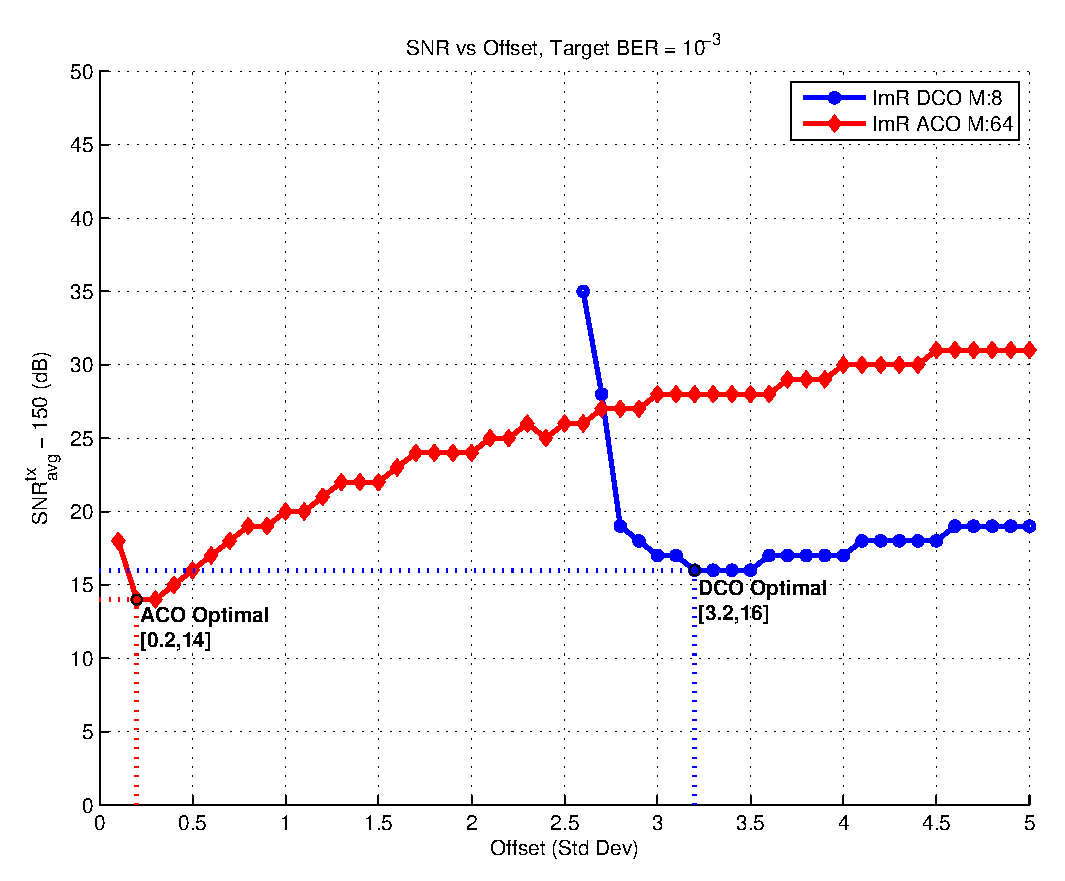
\includegraphics[trim={0.45in 0.25in 0.7in 0.0in}, clip=false, width=5in]{figSNRvsOfst.eps}
\caption{SNR vs Offset for target BER$= 10^{-3}$ using an ImR}
	\label{fig:SNRvsOfst}
\end{figure}

Different SIS-OFDM systems are compared at their optimal DC offsets as empirically determined from \figurename{\ref{fig:SNRvsOfst}}. BER vs SNR curves at optimal DC offsets equal to $0.2\times$SD for ACO-OFDM with 64-QAM subcarrier modulation and $3.2\times$SD for DCO-OFDM with 8-QAM subcarrier modulation using ImR and NImR are illustrated in \figurename{\ref{fig:BERnet}}. It is shown that using ImR can provide significant SNR gain ($\approx$135dB) over NImR for BER$=10^{-3}$. For the NImR, each photodiode receives significant signal from each of the 4 luminaires and thus high ICI is expected. The ImR provides channel decorrelation thus significantly improving the system performance. As seen from the figure, it is impractical to achieve $\approx$150dB SNR for SIS-OFDM with NImR. The above SIS-OFDM configurations are compared with reference SISO O-OFDM systems. To achieve nearly the same bits/symbol as in the SIS-OFDM systems, DCO-OFDM with 128-QAM subcarrier modulation and ACO-OFDM with 128$^2$-QAM subcarrier modulation yielding 217 and 224 bits/symbol are required. It is impractical to achieve $\approx$30dB SNR to achieve target BER performance at comparable spectral efficiencies for SISO O-OFDM systems with higher order subcarrier modulation. The SIS-OFDM system with ImR not only provides better spectral efficiency but also achieves the target BER at lower transmit powers. Additionally, the ImR considered has practical dimensions and can be incorporated in portable devices.

BER vs SNR curves for individual O-OFDM and OSM streams for the SIS-OFDM systems considered are shown in \figurename{\ref{fig:BERsplit}}. At low SNR, bit errors are dominated by errors in luminaire index detection. Errors in luminaire index leads to choosing a different signal value for decoding the O-OFDM signal, thus introducing additional errors in O-OFDM signal decoding. As the SNR increases, errors in transmitter index detection significantly decrease and errors in O-OFDM symbol decoding dominates the BER. As the SNR is further increased, errors in the O-OFDM symbol decoding decrease thus reducing the overall BER.
\begin{figure}[!t]
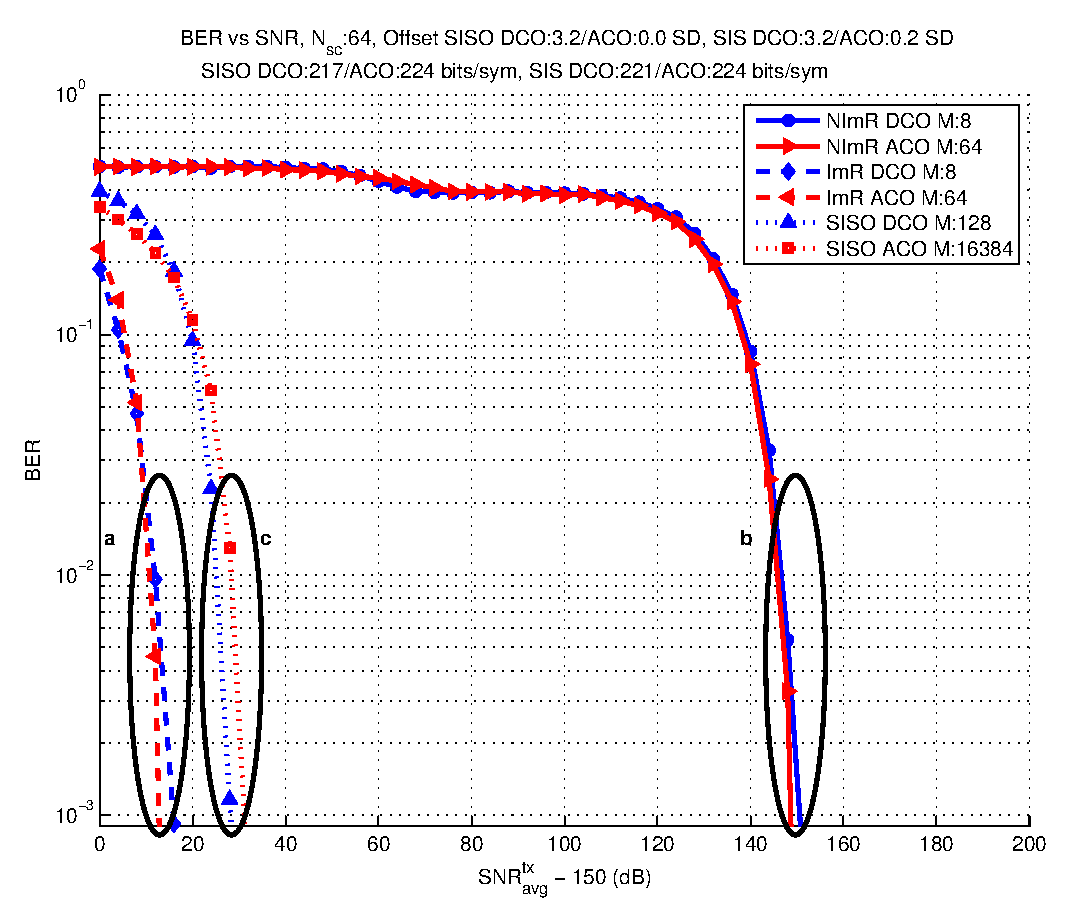
\includegraphics[trim={0.45in 0.15in 0.7in 0.00in}, clip=false, width=5in]{fig_35_64_all.eps}
\caption{Comparison of BER vs SNR for (a) ImR, (b) NImR and (c) SISO}
	\label{fig:BERnet}
\end{figure}
\begin{figure}[!t]
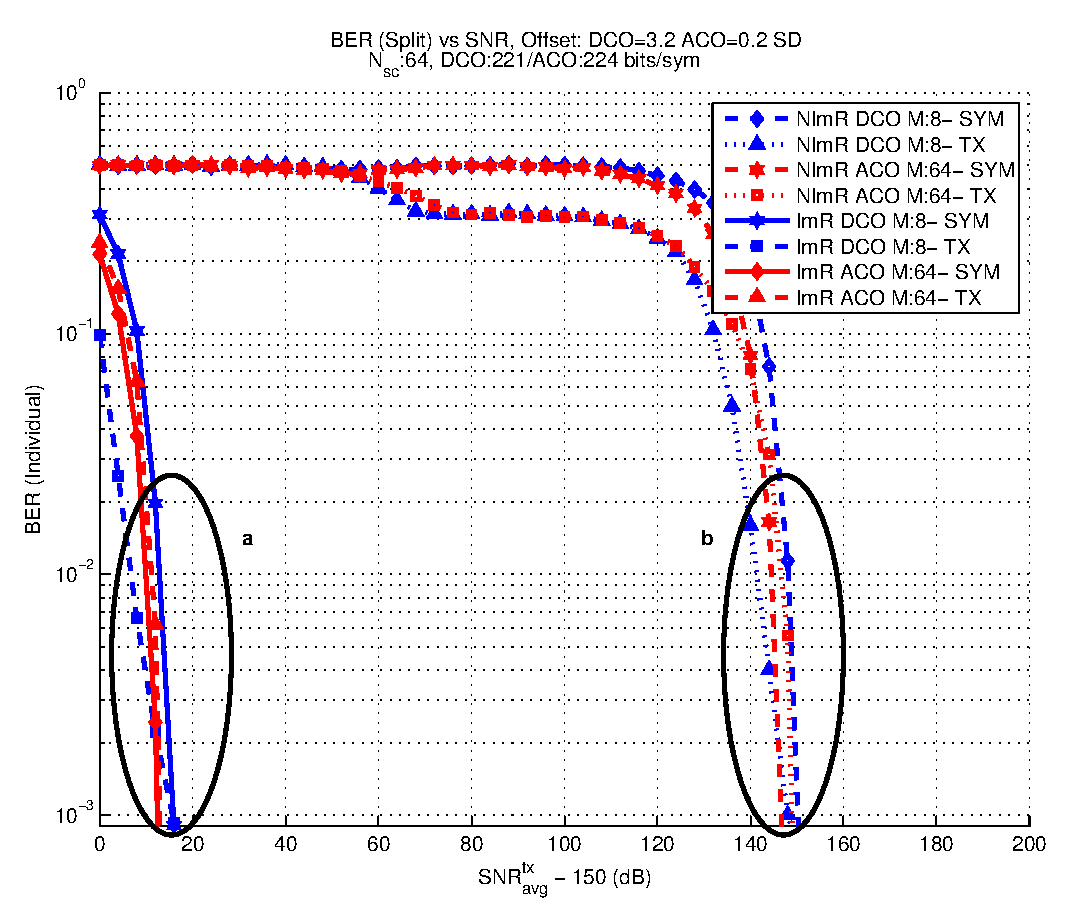
\includegraphics[trim={0.45in 0.15in 0.7in 0.00in}, clip=false, width=5in]{fig_35_64_all_s.eps}
\caption{Comparison of individual BER vs SNR for (a) ImR and (b) NImR}
	\label{fig:BERsplit}
\end{figure}

In conclusion, we show that a system implementing SIS-OFDM can achieve additional $R^s=N_{sc}\times log_2(N_{tx})$ bits per symbol of spectral efficiency as compared to SISO O-OFDM systems. Results indicate that the use of an ImR provides additional channel decorrelation and can help achieve up to 130dB improvement in SNR when compared to system performance using a NImR. At significantly lower computational complexity, the SIS-OFDM can provide an additional ($3\times N_{sc}\times k/4$) bits per symbol for ACO-OFDM and $((N_{sc}/2 -1)\times k)$ bits per symbol for DCO-OFDM over recently proposed approaches that combine OSM with O-OFDM.

\cleardoublepage